% !TEX root =  ../master.tex
\chapter{Nutzerhandbuch} 
Bei der Endwicklung der Anwendung haben wir großen Wert auf eine intuitive Gestaltung des \ac{GUI} und der \ac{UX} gelegt. Ziel war es, eine Anwendung zu gestalten, deren Nutzer die Anwendung ohne Erklärung verstehen können.
Dennoch möchten wir in diesem Kapitel ein Referenzhandbuch erstellen.
In diesem Kapitel wird beschrieben, wie Nutzer die Anwendung handhaben können.

\section{Öffnen der Anwendung}
Die Anwendung kann jederzeit unter \href{https://dhbwlearning.web.app}{\enquote{dhbwlearning.web.app}} geöffnet werden.
Wie bei jeder anderen Webapplikation kann sie über jedes Gerät, welches über eine Internetverbindung verfügt, durch einen Webbrowser geöffnet werden. Das heißt, die Anwendung steht 24\,h pro Tag bereit und kann von allen Studenten und Dozenten rund um die Uhr verwendet werden.

\section{Login}
Nach dem Öffnen der Anwendung wird der Nutzer in der Regel aufgefordert sich einzuloggen.
In \autoref{fig:login} ist die Anmeldeseite dargestellt.

\begin{figure}[h]
    \centering
    \includegraphics[width=.7\textwidth]{img/Login.png}
    \caption{Login-Maske}
    \label{fig:login}
\end{figure}

Für die Anmeldung muss der Nutzer die Email-Adresse zu seinem Account sowie das entsprechende Passwort eingeben.
Setzt der Nutzer einen Hacken bei \enquote{Remember me}, so wird der Nutzer beim nächsten Starten der Anwendung nicht um ein Passwort gebeten und wird automatisch in seinen Account eingeloggt.

Sollte der Nutzer noch keinen Account haben, kann er auf \enquote{Hier gehts zur Registrieurng} klicken, um sich selbst für die Nutzung der Anwendung zu registrieren.
Genaueres zur Registrierung ist in \autoref{sec:registrierung} beschrieben.

Sollte der Nutzer bereits einen Account haben und nur das Passwort zu diesem vergessen haben, gibt es neben dem Passwort-Feld einen \enquote{Passwort vergessen?}-Button.
Dieser leitet den Nutzer zu einem Passwort-Vergessen-Formular weiter, welches in \autoref{sec:passwordVergessen} beschrieben wird.

Hat der Nutzer eine korrekte Email- und Passwortkombination eingetragen und auf \enquote{Login} geklickt, wird der Nutzer auf das Dashboard (vgl. \autoref{sec:dashboard}) weitergeleitet.
Andernfalls wird der Nutzer freundlich darauf hingewiesen, dass das Passwort nicht korrekt ist.



\section{Registrierung}\label{sec:registrierung}
Die Registrierungs-Maske dient dazu, einen neuen Nutzer in der Anwendung anzulegen.
Damit sich Nutzer registrieren können müssen sie eine Email-Adresse sowie ein Passwort wählen.
Der Nutzer kann hierbei eine beliebige, sogar eine Wegwerf-Email verwenden.
Die Email wird intern lediglich für Authentifizierungszwecke benötigt.
Das heißt die Email wird nur für das Login und für den Fall, dass ein Nutzer sein Passwort vergessen hat, benötigt (vgl \autoref{sec:passwordVergessen}).
Verwendet der Nutzer eine Wegwerf-Email, kann er die Anwendung wie gewohnt nutzen, verliert aber die Möglichkeit sein Passwort zurückzusetzen.

Das Passwort kann frei gewählt werden, solange es mindestens 6 und maximal 50 Zeichen hat.
Es gibt keine weiteren Einschränkungen, da wir der Meinung sind, dass aufwändige Passwortvorgaben eine schlechte \ac{UX} ergeben.
Dennoch sollten Nutzer Passwörter verwenden, die allgemein als sicher gelten. Dies bringt zusammen mit dem genutzten OAuth 2.0 Standard eine hohe Sicherheit mit sich. Um zu verhindern, dass sich der Nutzer bei seinem Passwort vertippt hat, muss das Passwort ein zweites Mal bestätigt werden.

Schließlich muss der User den Nutzungsbedingungen zustimmen.

Sollte der Nutzer bereits einen Useraccount besitzen, kann er jederzeit durch einen Klick auf \enquote{Log in} zur Login-Maske zurückkehren.

Ist alles korrekt ausgefüllt, kann der Nutzer durch einen Klick auf \enquote{Registrieren} die Anmeldung abschließen und wird automatisch eingeloggt.

Direkt nach der Registrierung wird der Nutzer auf eine Seite mit verschiedenen Fragen weitergeleitet. Diese Seite beinhaltet Fragen zu seinem Lerntypen. 
Der Nutzer kann die Fragen freiwillig beantworten. Sie helfen dem Dozenten, einen Überblick zu bekommen, welche verschiedenen Lerntypen in seinem Kurs enthalten sind und ermöglichen so die Adaption der Vorlesung und der angewannten Methoden an die Wünsche und Interessen des Kurses. Die Auswertung der Lerntypen wird unter dem Punkt \autoref{sec:Feedback} weiter behandelt.

\begin{figure}[h]
    \centering
    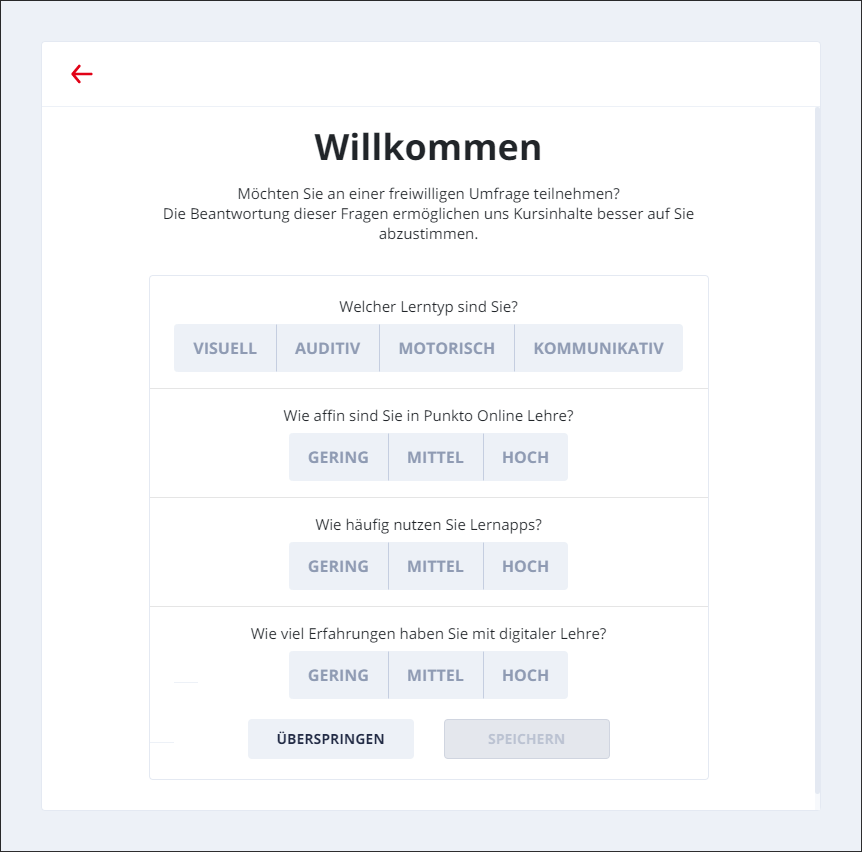
\includegraphics[width=.7\textwidth]{img/Einstiegsfragen.png}
    \caption{Einstiegsfragen}
    \label{fig:einstiegsfragen}
\end{figure}


\section{Passwort-Vergessen}\label{sec:passwordVergessen}
Die Passwort-Vergessen-Funktion dient zum Zurücksetzen des Passwortes.
Möchte der Nutzer sein Passwort zurücksetzen und erneut Zugang zu seinem Account bekommen, kann der Nutzer jederzeit seine Email in das Passwort-Vergessen-Feld eingeben.

\begin{figure}[h]
    \centering
    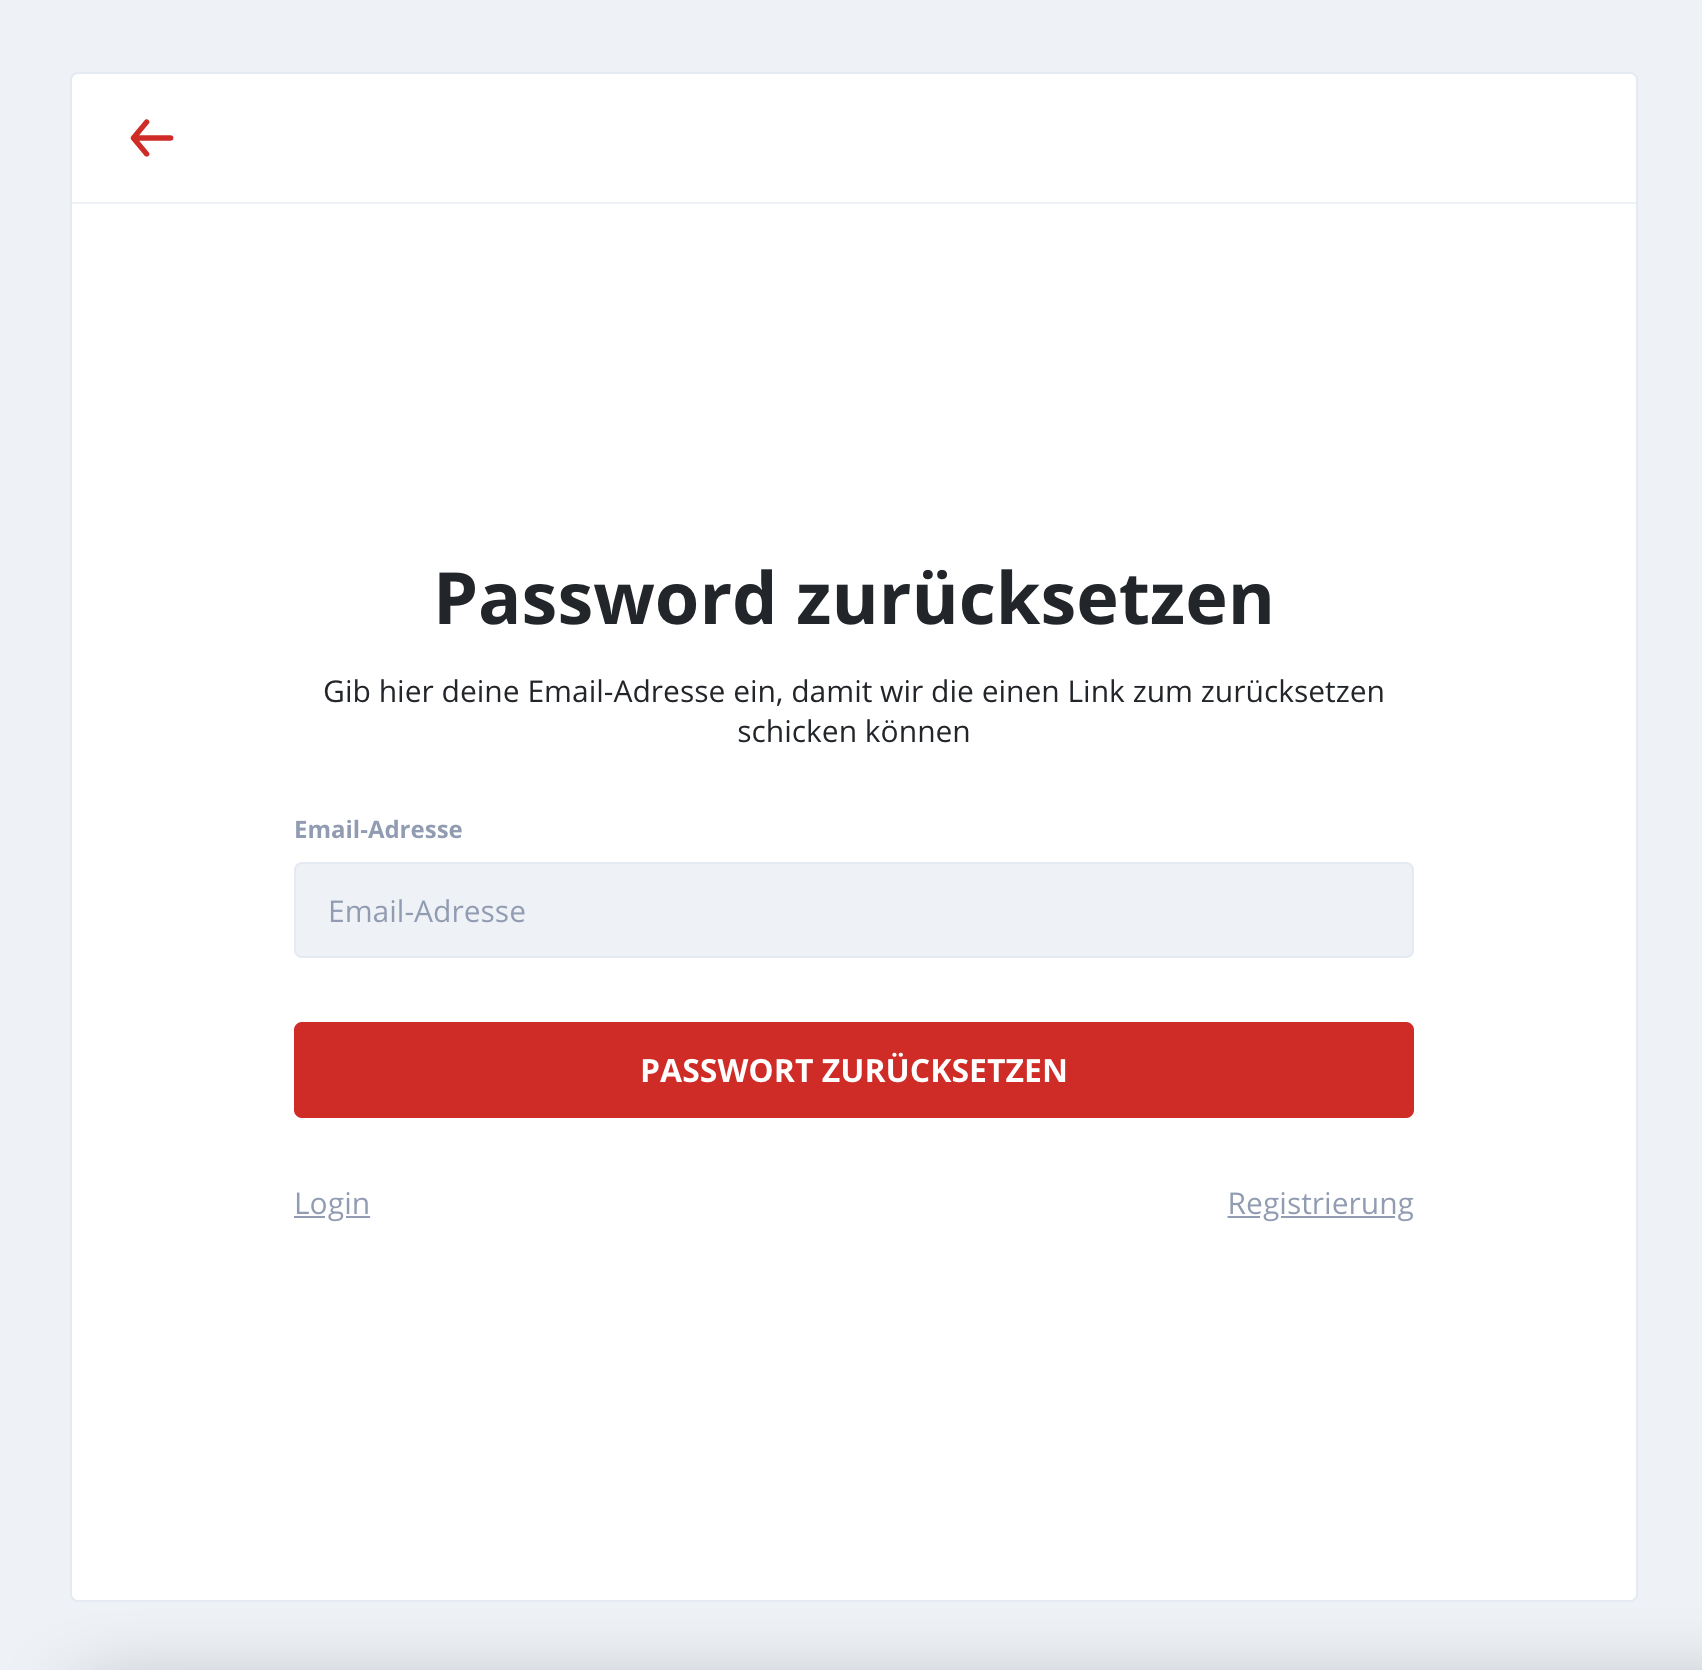
\includegraphics[width=.7\textwidth]{img/Passwort_zuruecksetzen.png}
    \caption{Passwort-Vergessen-Maske}
    \label{fig:passwordVergessen}
\end{figure}

Nachdem der Nutzer auf \enquote{Request Passwort} geklickt hat wird automatisch eine Email an die angegebene Email-Adresse gesendet.
Die Email enthält einen Link, mit dem der Nutzer sein Passwort ändern kann.
Der Link leitet den Nutzer auf die in \autoref{fig:passwordVergessen} dargestellte Maske, in der der Nutzer ein neues  Passwort festlegen kann. Hat der Nutzer sein Passwort erfolgreich geändert, wird er zu einem erneuten Login auf die Login-Maske geleitet.

Anzumerken ist, dass der Link zum ändern des Passworts nur einmal gültig ist.
Sollte das Passwort bereits geändert worden sein, muss eine neue Email angefordert werden.
Dies verhindert, dass unberechtigte Personen, welche die Email mitgelesen haben, das Passwort erneut ändern können.


\begin{figure}[h]
    \centering
    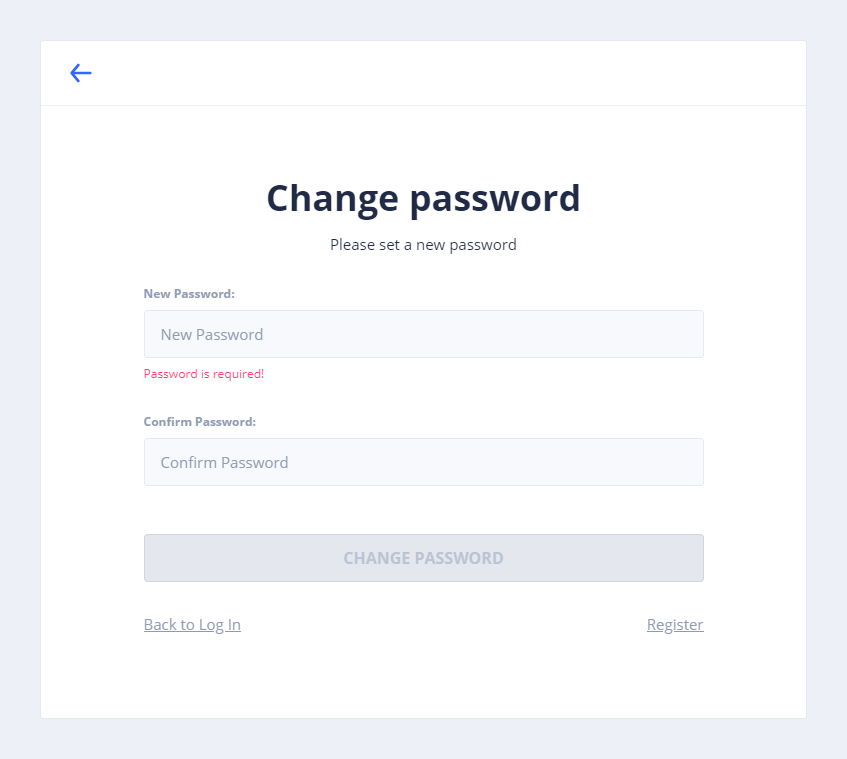
\includegraphics[width=.7\textwidth]{img/passwordReset2.png}
    \caption{Passwort-Aktualisieren-Maske}
    \label{fig:passwordVergessen2}
\end{figure}

\section{Dashboard}\label{sec:dashboard}
Das Dashboard ist die erste Seite, die der Nutzer sieht, wenn er sich erfolgreich eingeloggt hat. Es gibt einen Überblick über alle bevorstehenden Ereignisse.
Die nächsten anstehenden Prüfungen werden in einem Kalender angezeigt und auch die Gesamtanzahl an Prüfungen wird eingeblendet. In der Übersicht können nochmal die wichtigsten 
Informationen zu der Prüfung eingesehen werden, beispielsweise die Uhrzeit und der Raum. 
\begin{figure}[h]
    \centering
    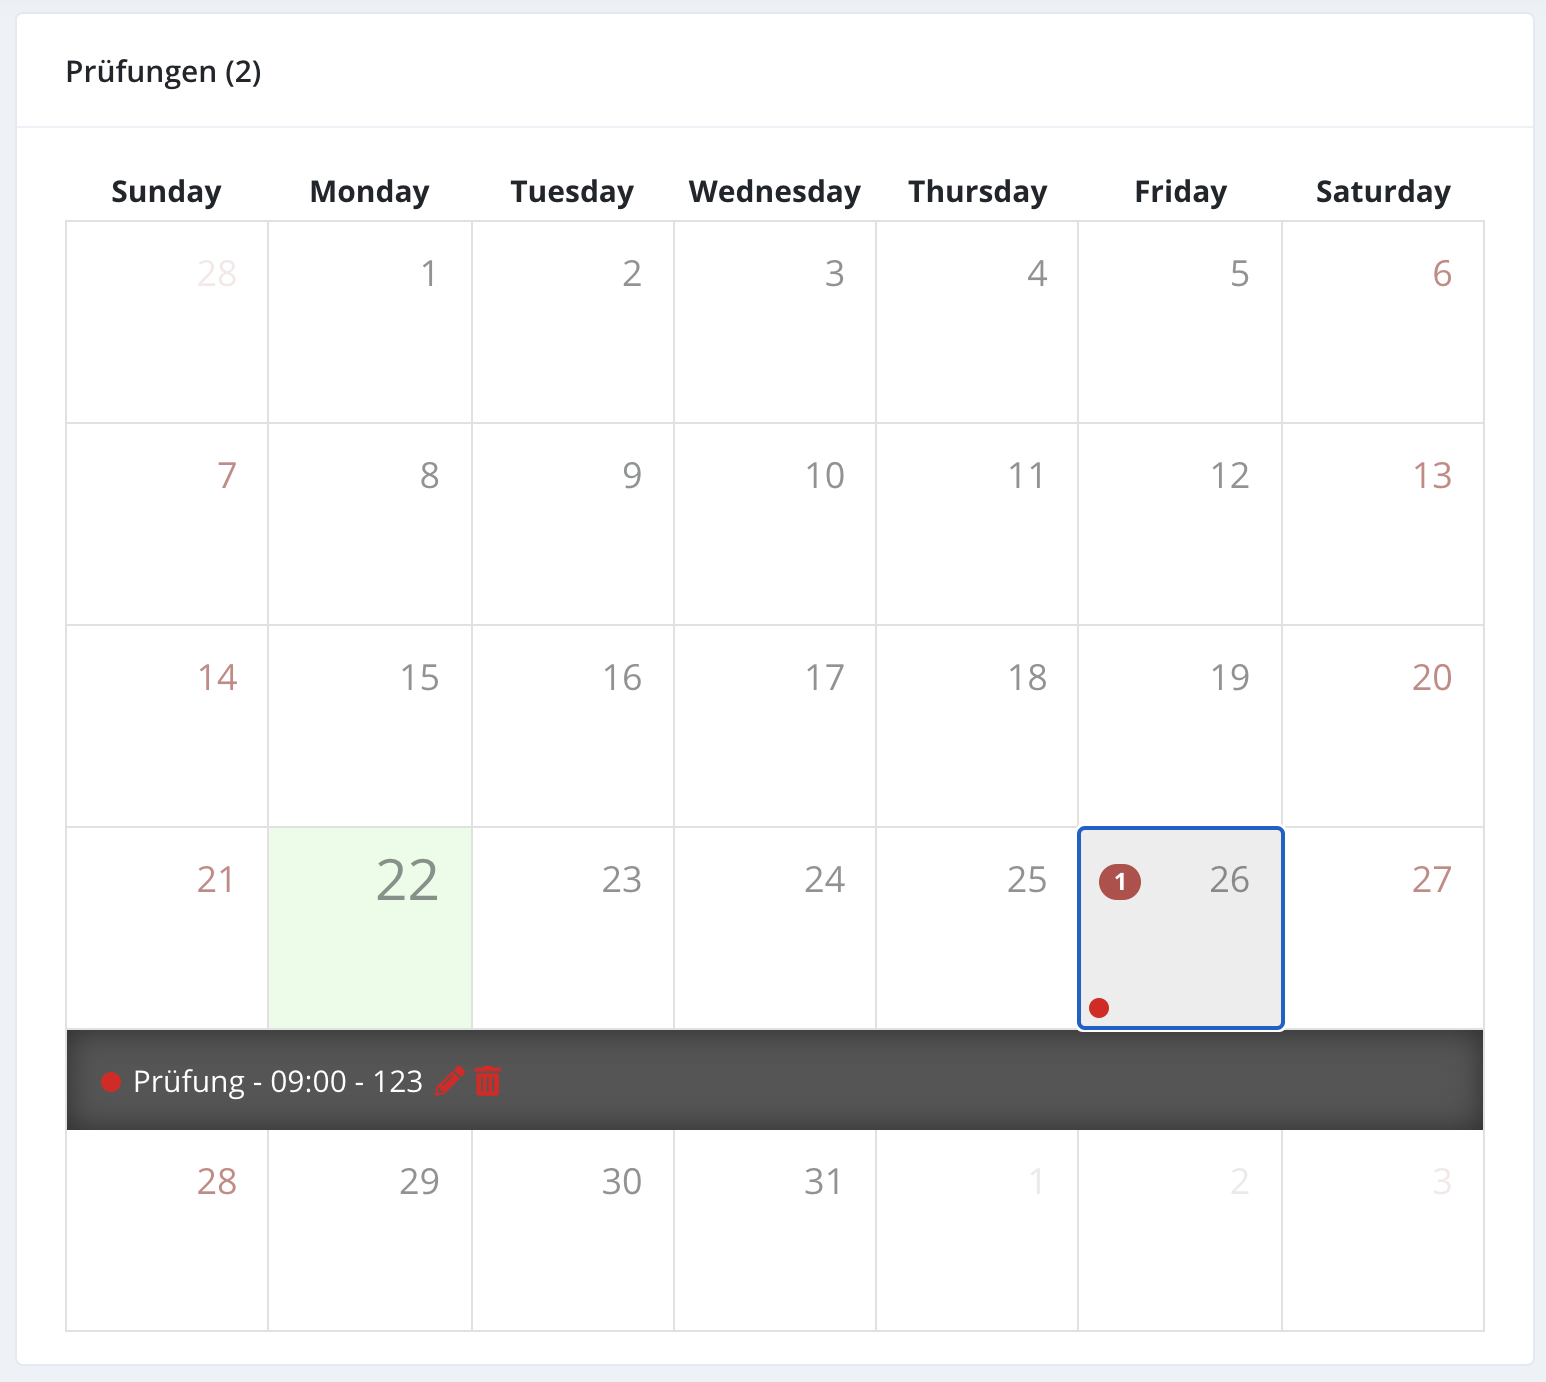
\includegraphics[width=.7\textwidth]{img/Dashboard_3.png}
    \caption{Dashboard-Prüfung}
    \label{fig:Dashboardansicht}
\end{figure}
Zusätzlich zu den nächsten Prüfungen werden auch bald fällige Aufgaben angezeigt. Der Nutzer sieht auf einen Blick, wie viele Tage er noch für welche Aufgabe hat.
\begin{figure}[h]
    \centering
    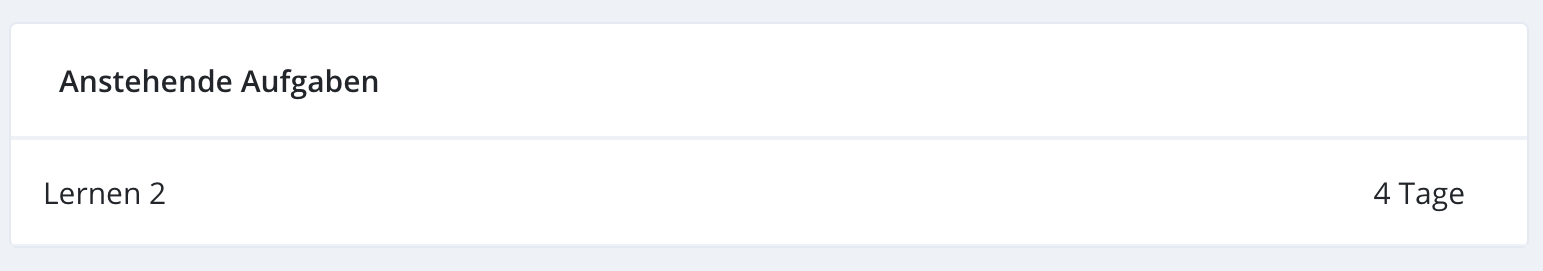
\includegraphics[width=.7\textwidth]{img/Dashboard_4.png}
    \caption{Dashboard-Aufgaben}
    \label{fig:Dashboardaufgaben}
\end{figure}

\section{Karteikarten}\label{sec:Karteikarten}
Index-Cards stellen eine Karteikarten-Funktion dar. Dabei können Dozenten neue Karteikarten erstellen, die die Kursteilnehmer dann bearbeiten können.
Im Nutzer-Interface werden diese Karten ähnlich zu einem realen Karteikasten hintereinander dargestellt.
Jede Karte zeigt zunächst die Frage an.
Sollte man die Antwort zu der Frage nicht wissen oder sich kontrollieren wollen, kann man mithilfe des Pfeils im Eck einer jeden Karte die Antwort einblenden.
Anschließend können die Karten mit den Buttons am unteren Bildschirmrand als gewusst oder nicht gewusst markiert werden.
Durch die Zahlen an diesen Buttons kann der Nutzer leicht ablesen, wie viele Karten er bereits wusste.
Karten können aber auch durch einfaches ziehen der Karten zu gewusst oder nicht gewusst verschoben werden.
Dies erleichtert die Handhabung vor allem auf mobilen Geräten mit Toucheingabe. In der Abbildung \autoref{fig:Karteikarten} ist die Ansicht zu sehen, die ein Teilnehmer bekommt, wenn er die Karteikarten durcharbeitet.
\begin{figure}[h]
    \centering
    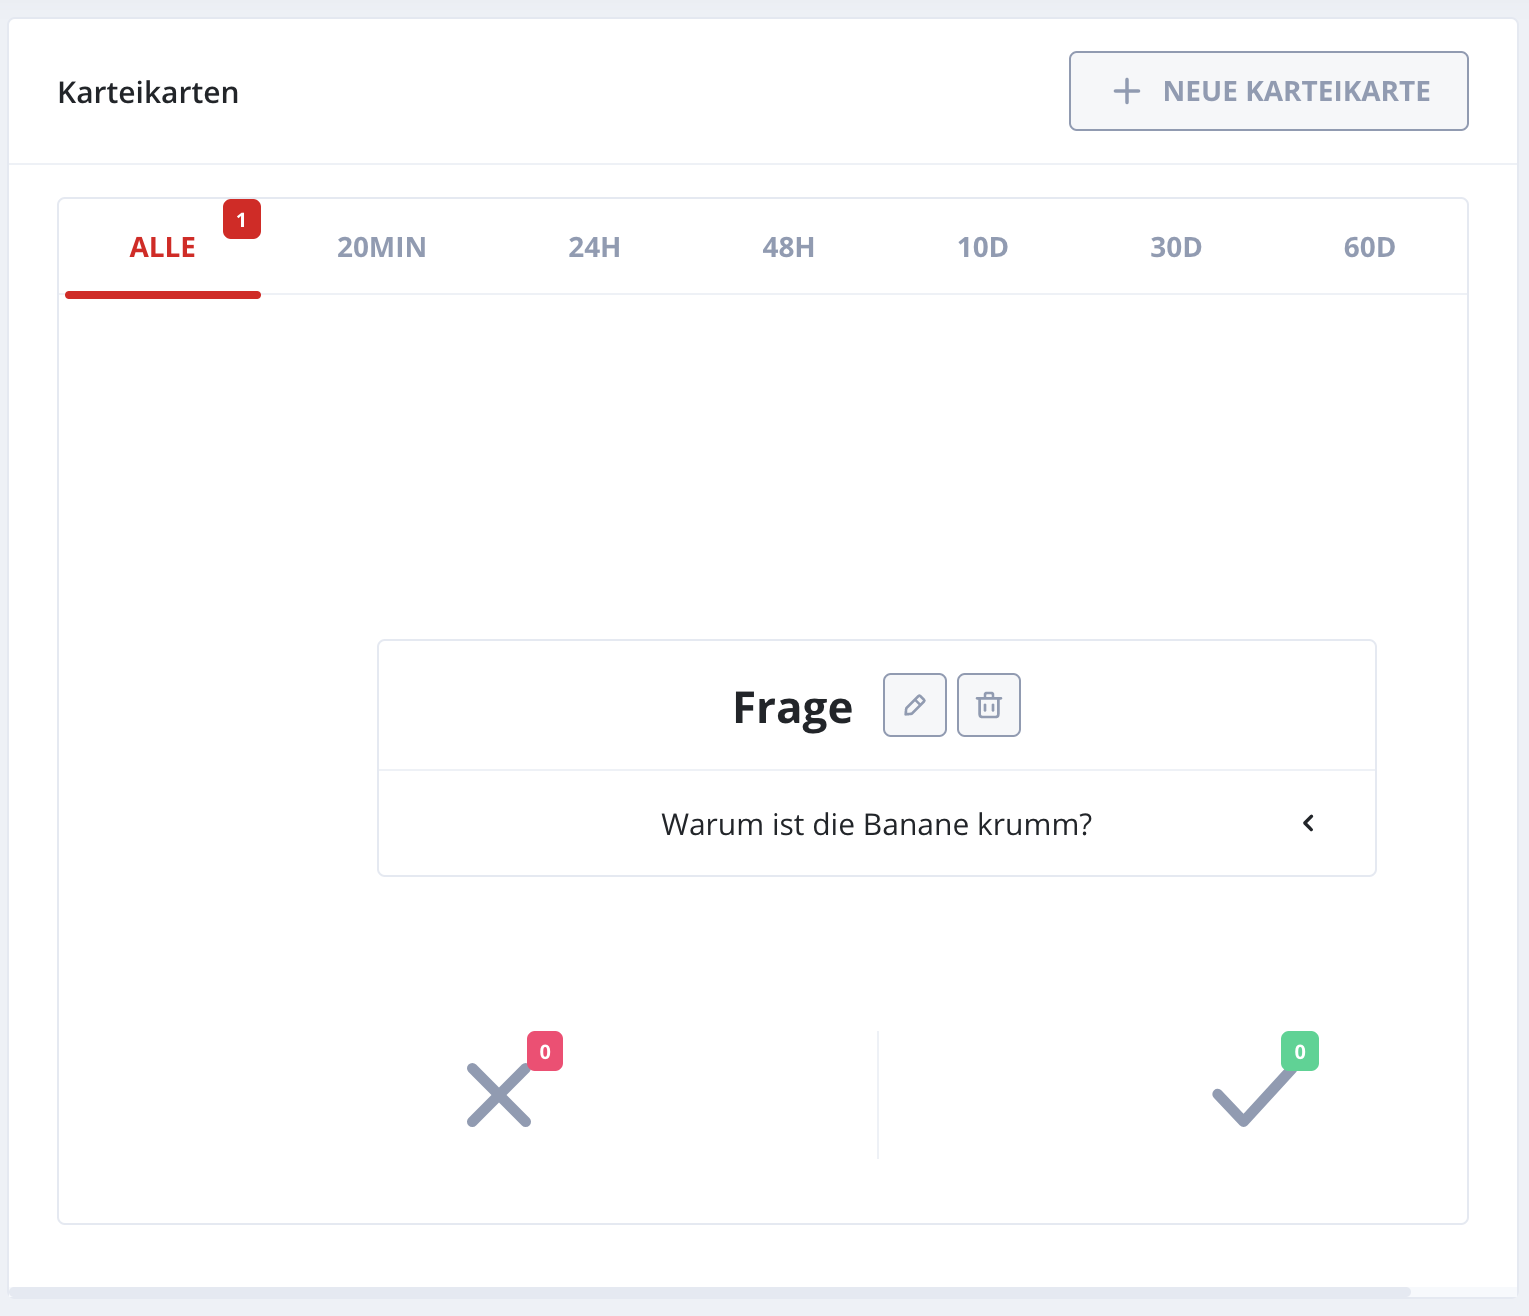
\includegraphics[width=.7\textwidth]{img/Karteikarten_hinzugefuegt.png}
    \caption{Karteikarten}
    \label{fig:Karteikarten}
\end{figure}

Wurden alle Karteikarten beantwortet bekommt der Student direkt Feedback, wie viel Prozent aller Fragen er richtig beantworten konnte. Durch die in den unterschiedlichen Registern angezeigten Zahlen hat er einen direkten Überblick, wie viele Karteikarten er noch einmal auffrischen sollte.


\section{Aufgaben}\label{sec:Aufgaben}
Aufgaben können mithilfe des Buttons im rechten unterem Eck erstellt werden.

Nach dem Klick öffnet sich ein Modul, in dem alle relevanten Aufgaben eingetragen werden können.
Aufgaben zeichnen sich durch einen Titel und eine optionale Beschreibung sowie eine optionale Deadline aus.
Sofern eine Deadline angegeben ist, wird dieses Aufgabe im Kalender über der Aufgaben-Übersicht dargestellt.
Je roter ein Tag ist, desto mehr Aufgaben müssen an diesem Tag erledigt sein.
Der Kalender zeigt stets den Zeitraum zwischen Anfang des letzten Monates und Ende der nächsten zwei Monate  an.

Aufgaben können schnell und einfach durch klicken auf die Checkbox vor einer Aufgabe abgehackt werden.
In \autoref{fig:Aufgabeanlegen} ist bereits eine Aufgabe angelegt und es ist zu sehen, in welchem Zeitraum diese Aufgabe erledigt werden muss.
\begin{figure}[h]
    \centering
    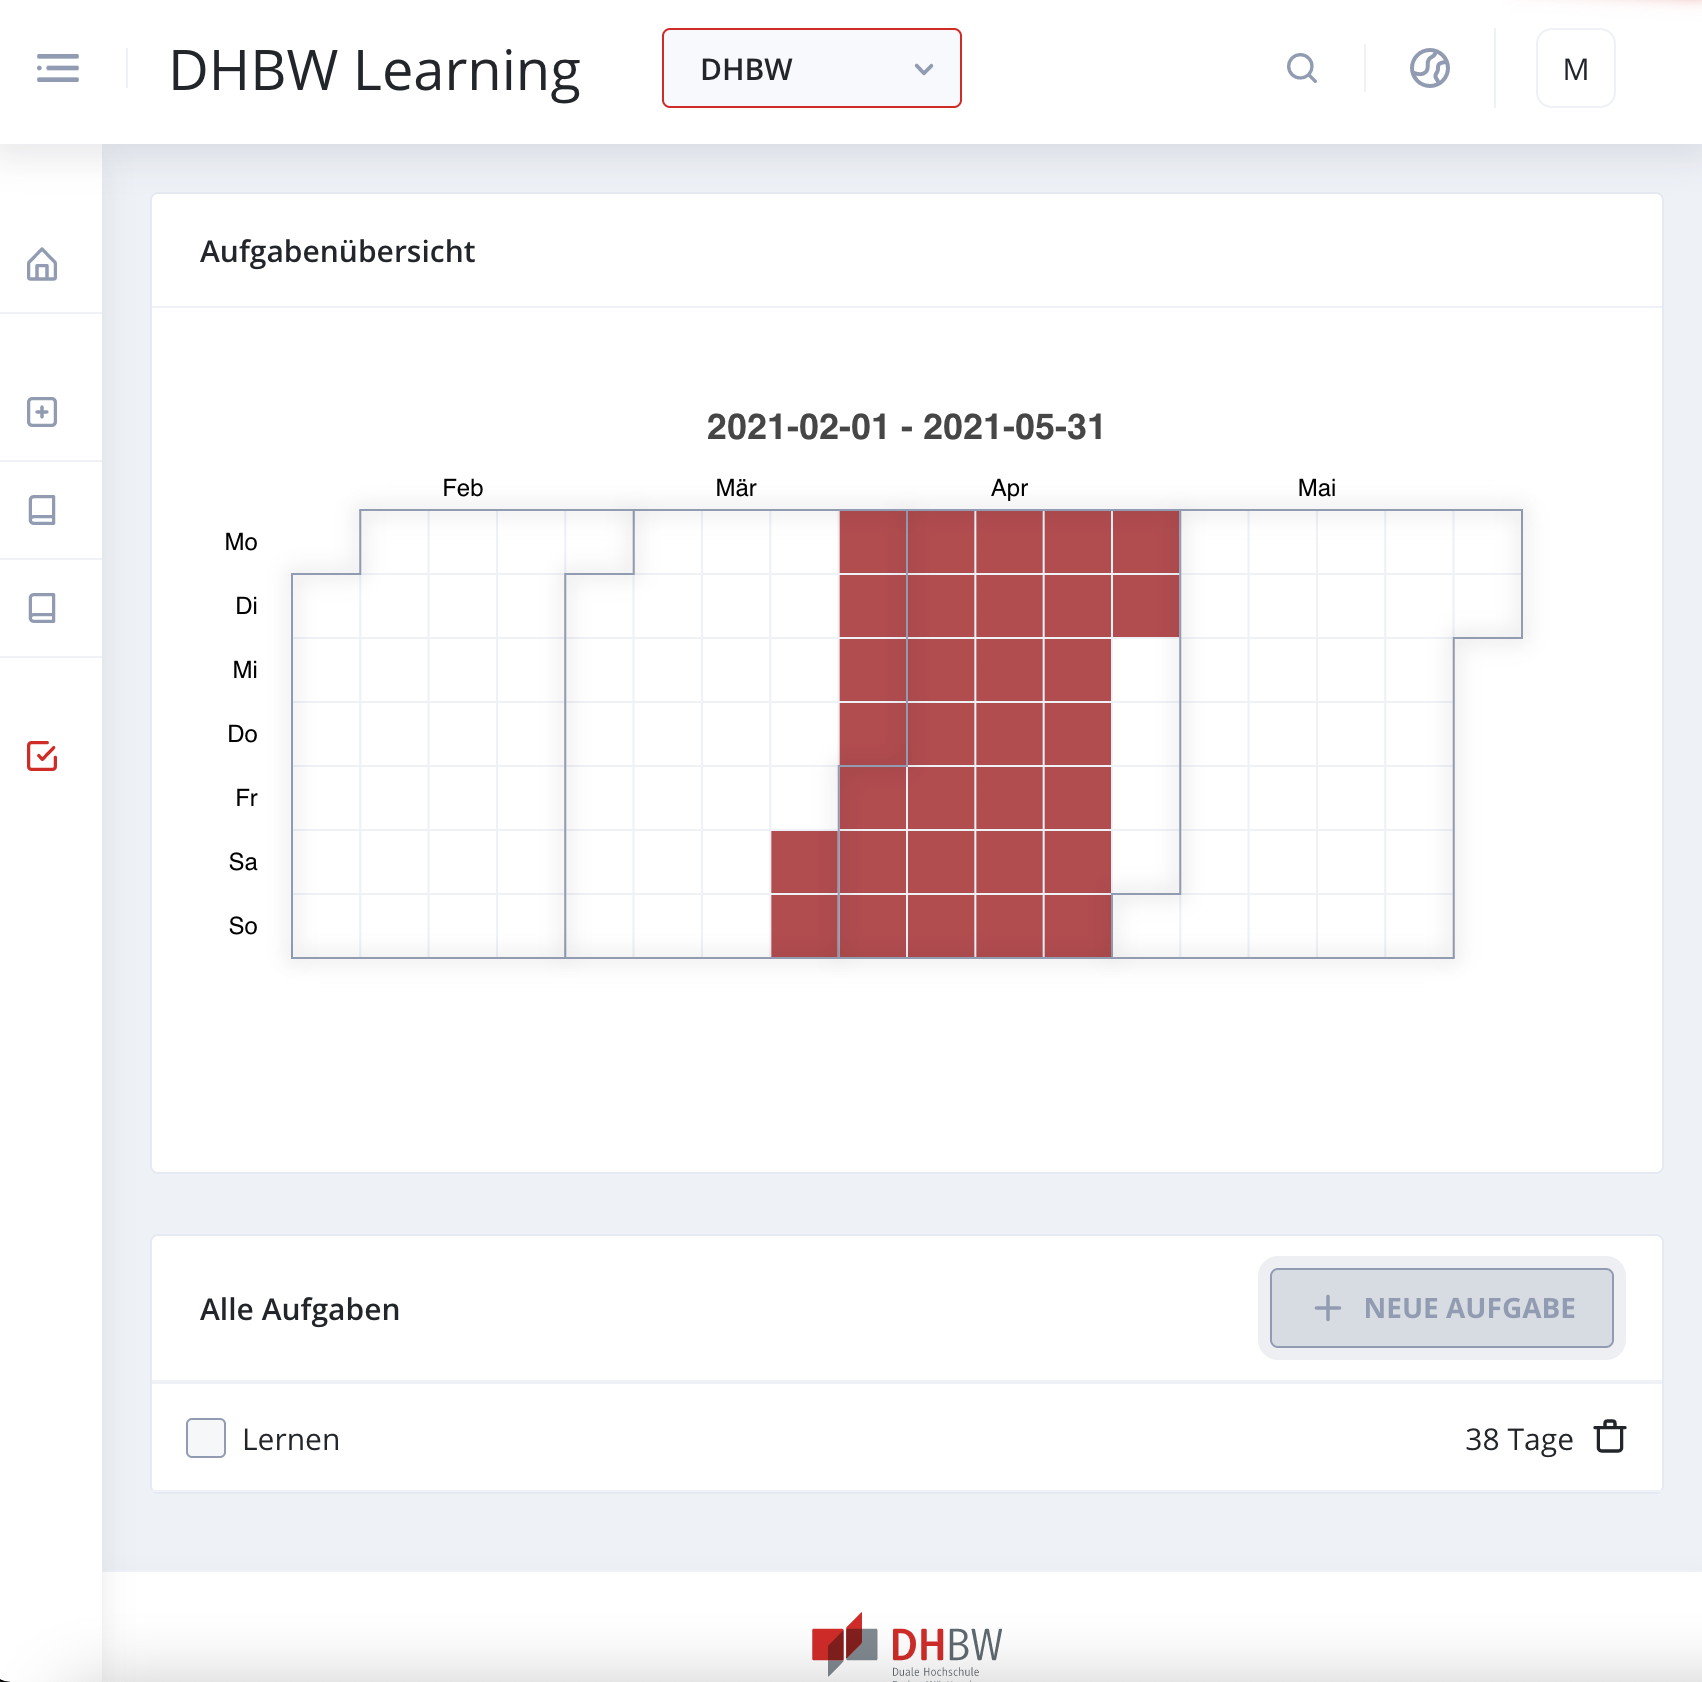
\includegraphics[width=.7\textwidth]{img/Aufgabe_angelegt.png}
    \caption{Aufgabe angelegt}
    \label{fig:Aufgabeanlegen}
\end{figure}




\section{Dateien}
Die \enquote{Dateien}-Maske dient zur Verwaltung von Dokumenten.

\begin{figure}[h] 
    \centering
    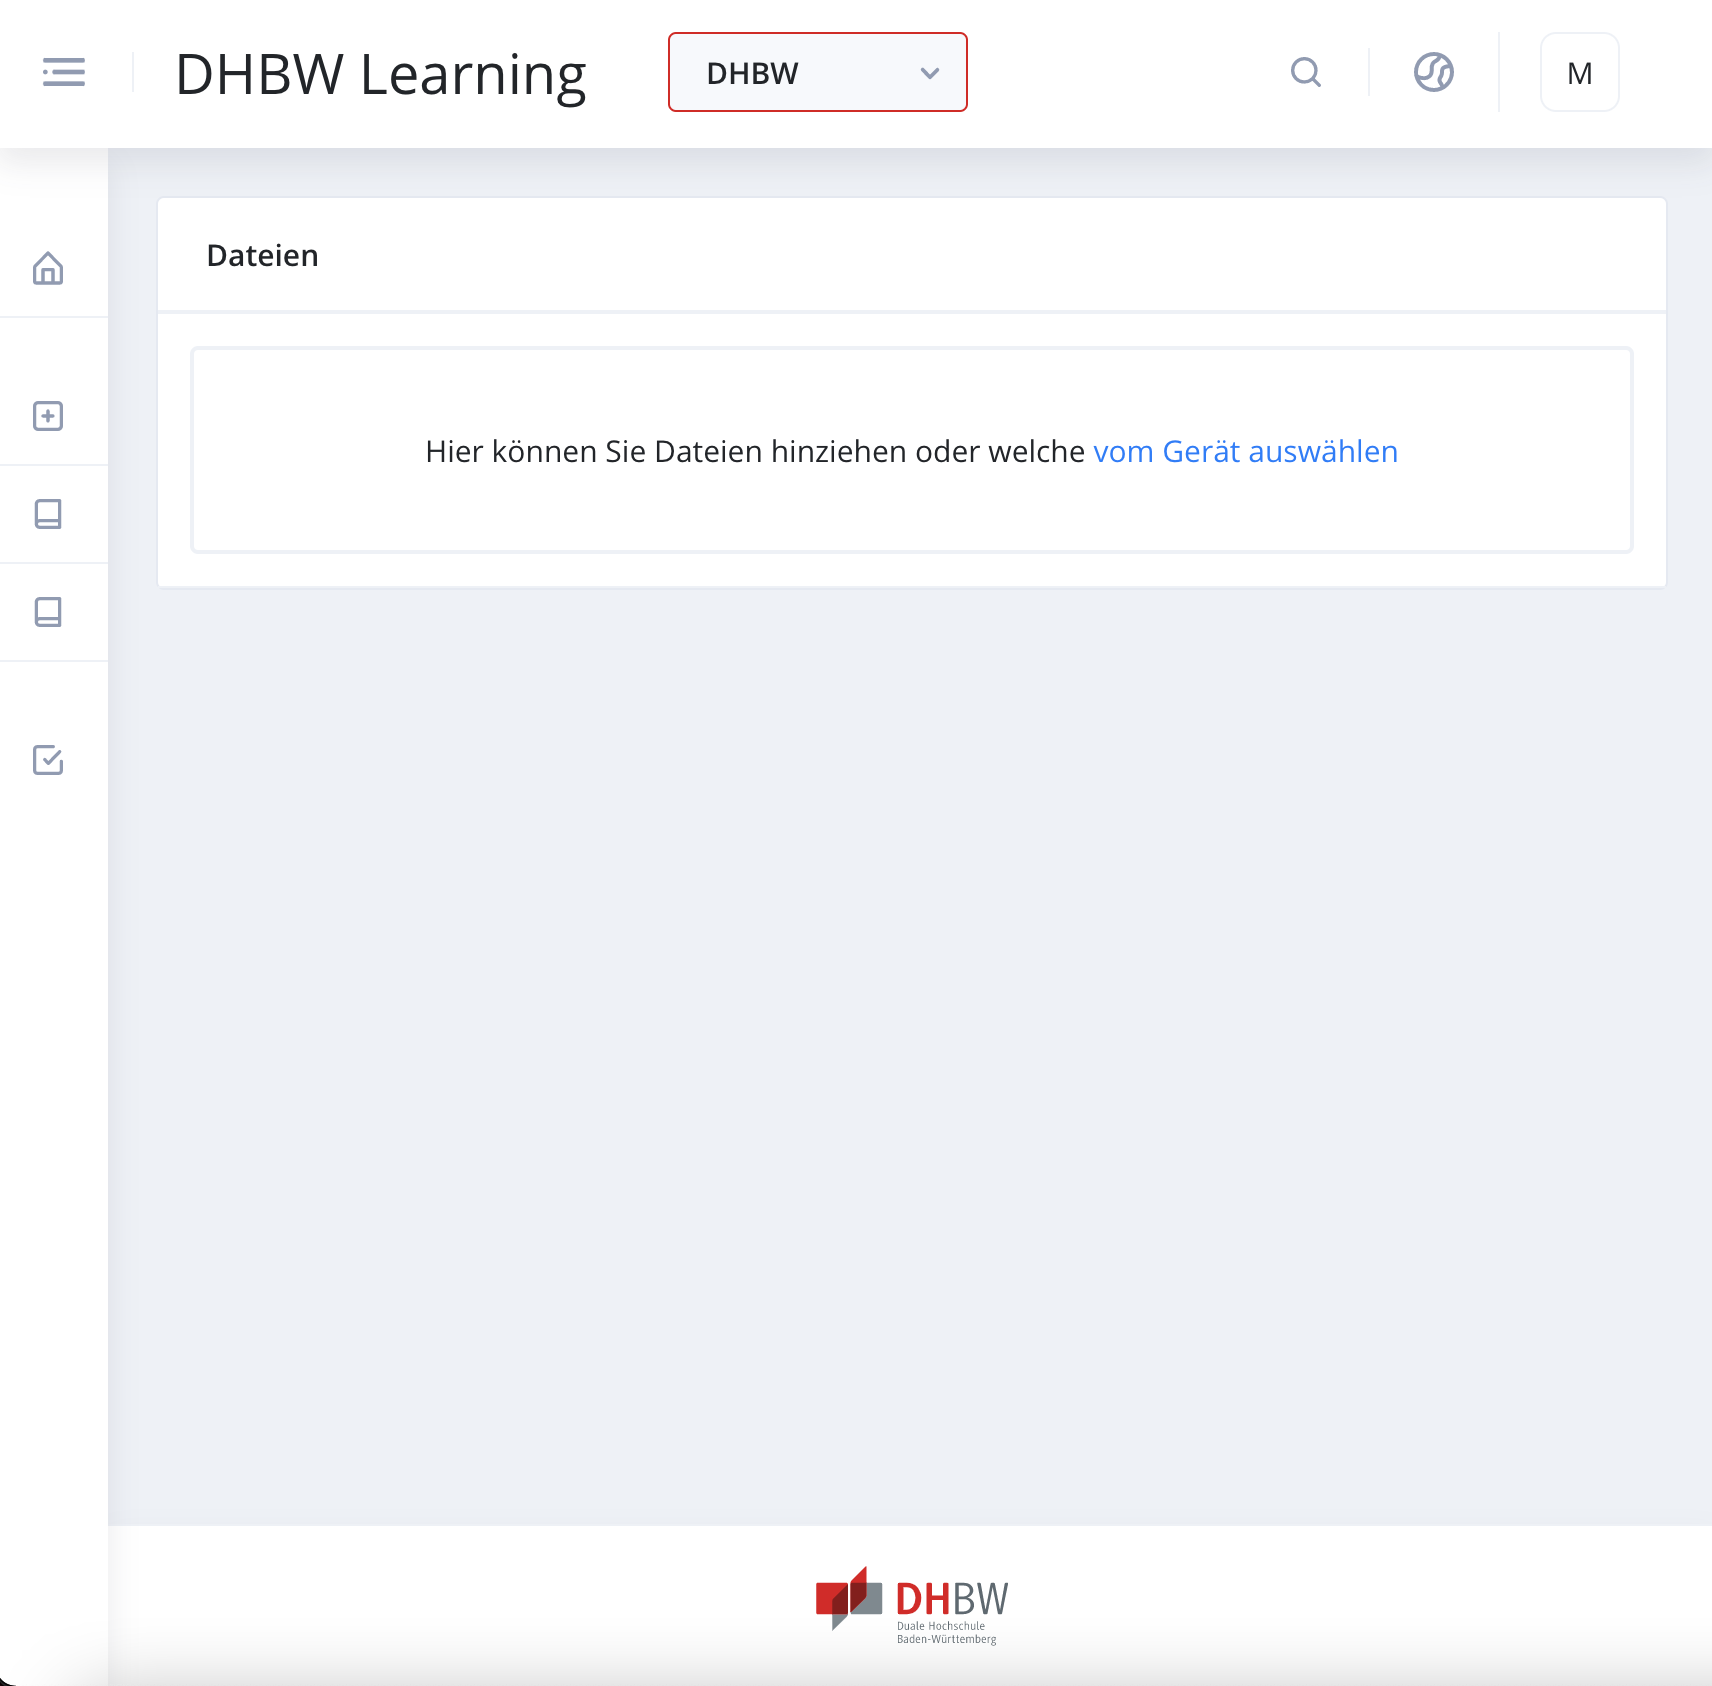
\includegraphics[width=.7\textwidth]{img/Dateien_uebersicht.png}
    \caption{Dateien-Maske}
    \label{fig:dateien}
\end{figure}

Das in \autoref{fig:dateien} dargestellte Datenmanagementsystem erleichtert dies, da Dokumente für einen Kurs hochgeladen werden können.
Dokumente können mithilfe des \enquote{browse}-Button hochgeladen werden.
Dafür öffnet sich ein Fenster, in dem beliebig viele Dateien für den Upload hochgeladen werden können.
Zur einfacheren Nutzung können optional auch Dateien direkt aus dem Explorer in das Fenster gezogen werden.

Anschließend werden die Dateien hochgeladen.
Ein Fortschrittsbalken zeigt dabei stets den aktuellen Upload-Fortschritt an.
Anschließend können die Dokumente von allen Studenten heruntergeladen werden.

Bei der Nutzung des Dateisystems ist darauf zu achten, dass aus Speichergründen nicht alle Dateien antizipierend heruntergeladen werden können. Dadurch könnten nämlich Geräte von Studenten überfordert werden.
Besonders Mobilgeräte besitzen noch einen begrenzten Speicher.
Aus diesem Grund muss während der Benutzung auf eine Internetverbindung geachtet werden.
Offline können nur die existierenden Dateien angezeigt werden, aber weder neue hochgeladen noch bestehende heruntergeladen werden.


Aus technischer Sicht werden mehrere Schritte unternommen, um die Dateiablage zu ermöglichen.
Sobald Dateien ausgewählt oder Dateien in das Fenster gezogen wurden, wird der Upload dieser Dateien zu FireStorage angestoßen.
Dabei handelt es sich um eine Bucket-basierte Speicherlösung ähnlich zu AWS S3.
Während des Uploads wird der Zustand überwacht, wieviel der Dateien bereits übertragen werden konnte.
Dieser Wert wird automatisch in den Fortschrittsbalken weitergeleitet, welcher sich dadurch reaktiv aktualisiert.


Konnte der Upload erfolgreich durchgeführt werden, wird der Fortschrittsbalken grün und eine Benachrichtigung informiert, dass die Datei erfolgreich hochgeladen werden konnte.
Im Hintergrund wird anschließend ein Datenbankeintrag getätigt, ab welchem Zeitpunkt andere Nutzer auf die Datei zugreifen können.

Wird eine Datei gelöscht, so wird der gleiche Vorgang rückwärts durchgeführt.
Das heißt, zuerst wird der Datenbankeintrag gelöscht, wodurch Studenten nicht mehr darauf zugreifen können.
Anschließend wird die eigentliche Datei aus dem Bucket-Speicher gelöscht.


\section{Feedback}\label{sec:Feedback}
Die Feedback-Maske dient dazu, einem Dozenten eine unmittelbare Rückmeldung zu geben, wodurch Dozenten jederzeit ihren Vorlesungsstil anpassen können.

Im Vergleich zu den Umfragen am Ende eines Semesters werden die Umfragen in der Anwendung kurz gehalten.
Dies geht daraus hervor, dass es als eine schnelle Feedbackmöglichkeit gedacht ist und eine kurze Umfrage die Chance erhöht, dass das Feedback ausgefüllt wird.
In der \autoref{fig:feedback} sind die verschiedenen Punkte aufgelistet, bei denen die Kursteilnehmer dem Dozenten Feedback geben können.
\begin{figure}[!h] 
    \centering
    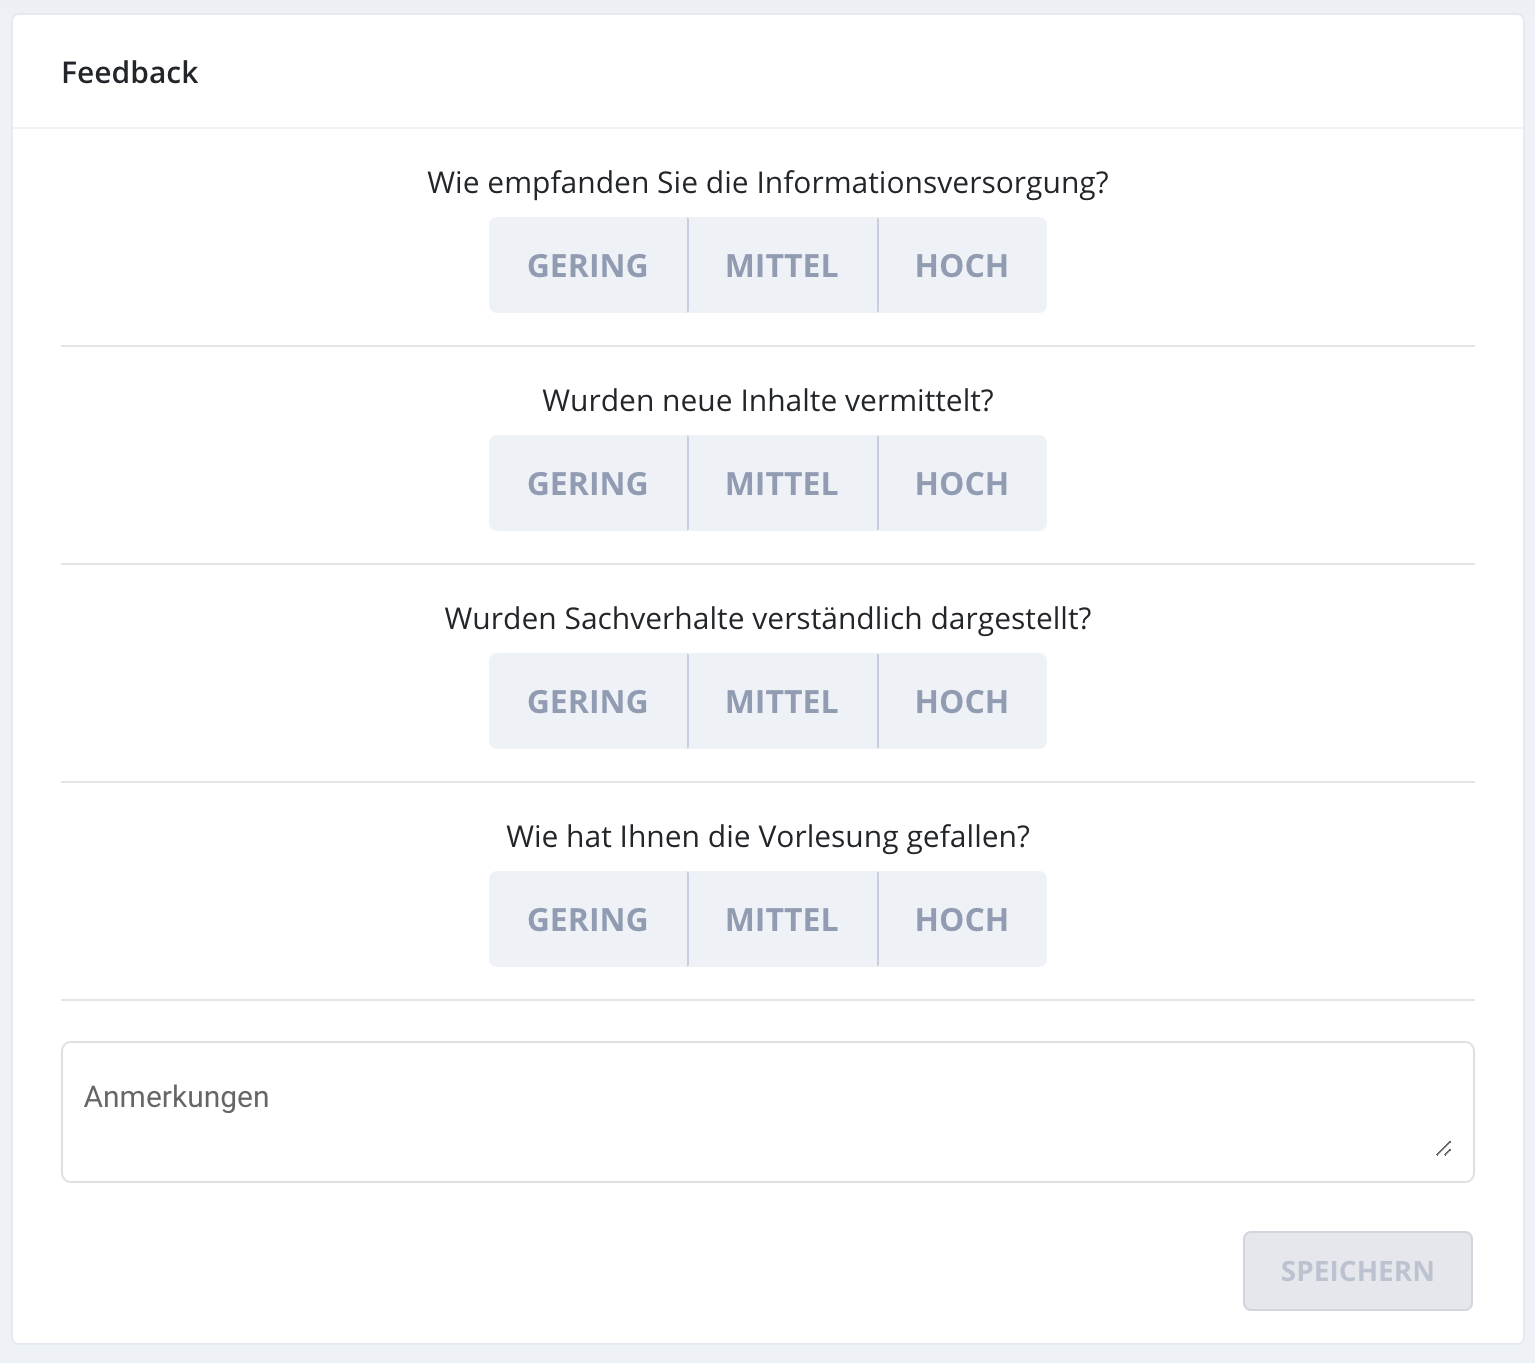
\includegraphics[width=.7\textwidth]{img/Feedback_geben.png}
    \caption{Feedback}
    \label{fig:feedback}
\end{figure}
Der Dozent kann, nachdem die Teilnehmer ihr Feedback gegeben haben, die Antworten auswerten. Zum einen kann diese Auswertung direkt in der Webapplikation vorgenommen werden, zum anderen können die Ergebnisse als CSV-Datei exportiert und selbstständig ausgewertet werden. In der \autoref{fig:feedback_ergebnis} 
wird eine beispielhafte Auswertung angezeigt.
\begin{figure}[!h] 
    \centering
    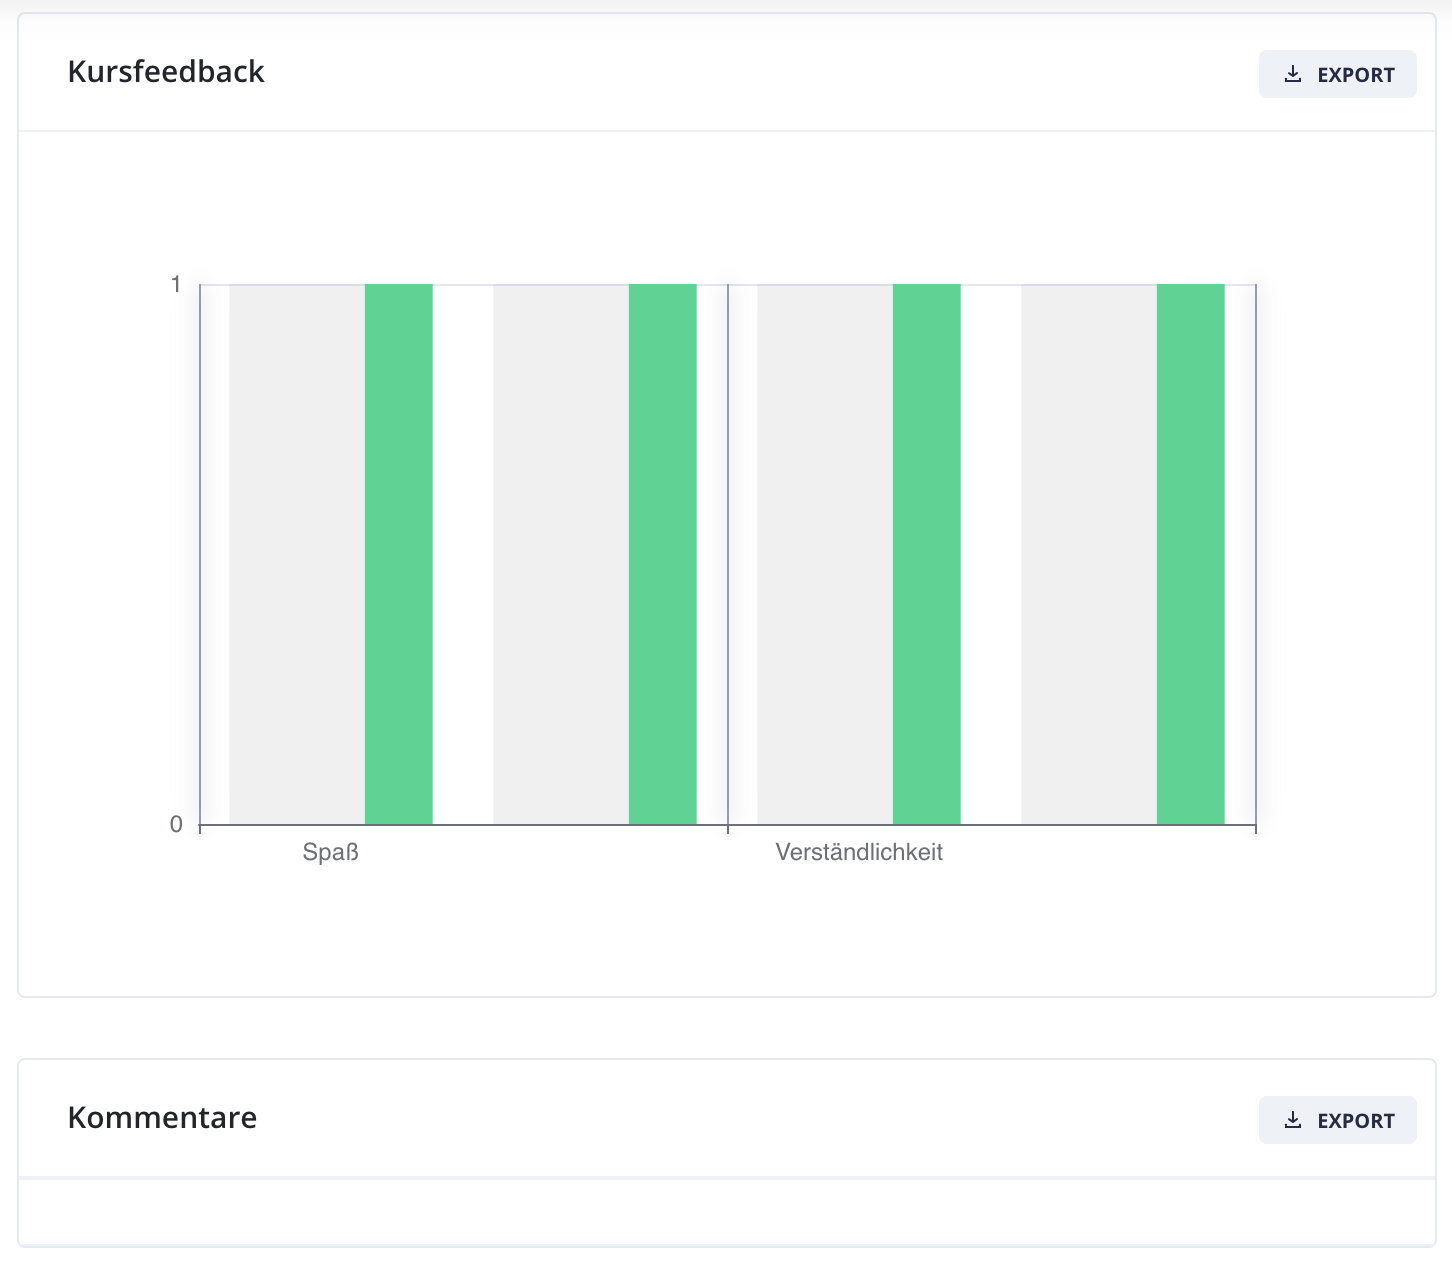
\includegraphics[width=.7\textwidth]{img/Feedback_uebersicht_Teilnehmer_Feedback.png}
    \caption{Feedback-Ergebnis}
    \label{fig:feedback_ergebnis}
\end{figure}
Als letztes Feature bei der Feedbackoption kann eine Übersicht zum Kurs angezeigt werden. Diese Übersicht beinhaltet alle Antworten zu den Fragen, die 
bei der Registrierung gestellt werden. Dadurch hat der Dozent einen Eindruck, welche Arten von Lerntypen in diesem Kurs vertreten sind und wie viel 
Erfahrung die Teilnehmer mit der Online-Lehre haben. 
\begin{figure}[!h] 
    \centering
    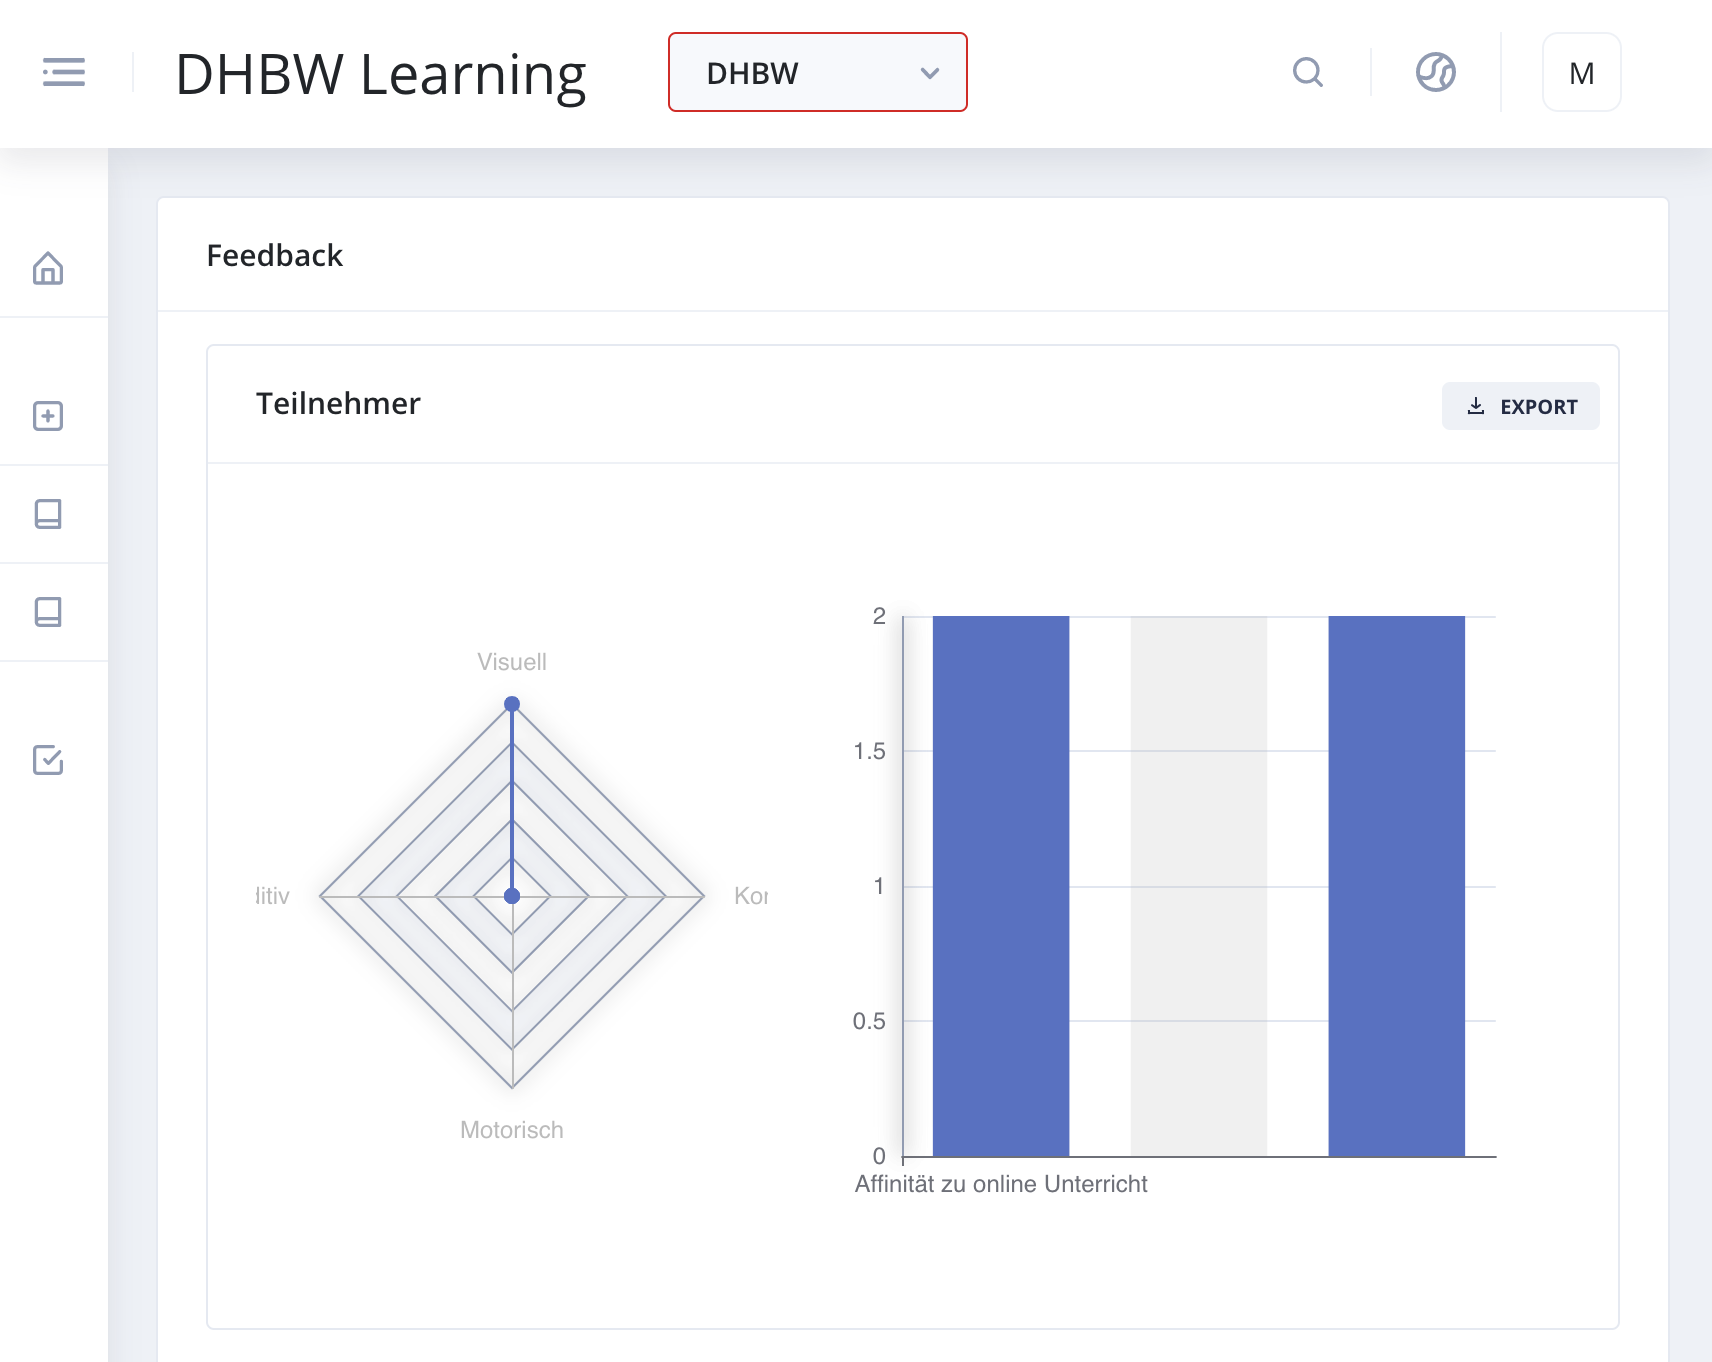
\includegraphics[width=.7\textwidth]{img/Feedback_uebersicht_Teilnehmer.png}
    \caption{Übersicht-Teilnehmner}
    \label{fig:uebersichtTeilnehmner}
\end{figure}

\section{Exams}
Als Studenten konnten wir ein weiteres Problem mit der aktuellen Informationsversorgung identifizieren.
Momentan herrscht eine große Unklarheit über Prüfungsleistungen.
Teilweise werden die Prüfungsleistungen in den Vorlesungen angekündigt, manche werden in Moodle und wieder andere in einem Google-Kalender eingetragen. Außer einem Datum sind oft keine weiteren Informationen festgeschrieben. Stattdessen werden diese mündlich in den Vorlesungen bekanntgegeben.
Besonders für Studenten, die Aufgrund von Krankheiten oder, in der Zeit von Online-Vorlesungen, Internetverbindungsprobleme erfahren und deshalb diese Informationen nicht mitbekommen, ist dies problematisch.

Insbesondere bei Portfolioprüfungen kommt hinzu, dass die Prüfungen nicht aus einer einzelnen, sondern aus mehreren Leistungen bestehen.
Ein Beispiel ist die Erstellung einer Präsentation, bei der nicht nur der Vortrag, sondern auch das Begleitmaterial bewertet wird.

Aus diesem Grund können in der Anwendungen Informationen zu Klausuren verwaltet werden.
Jede Prüfungsleistung besitzt einen Titel und einer Beschreibung, in der notiert werden kann, was die Aufgabe ist.
Außerdem wird das Abgabedatum in einem Kalender zur einfacheren Übersicht dargestellt.
Zusätzlich werden alle wichtigen Informationen, wie Räume oder zugelassenen Hilfsmittel, dargestellt.
Die Eingabemaske ist in der Abbildung \autoref{fig:pruefungsmaske} zu sehen.
\begin{figure}[h] 
    \centering
    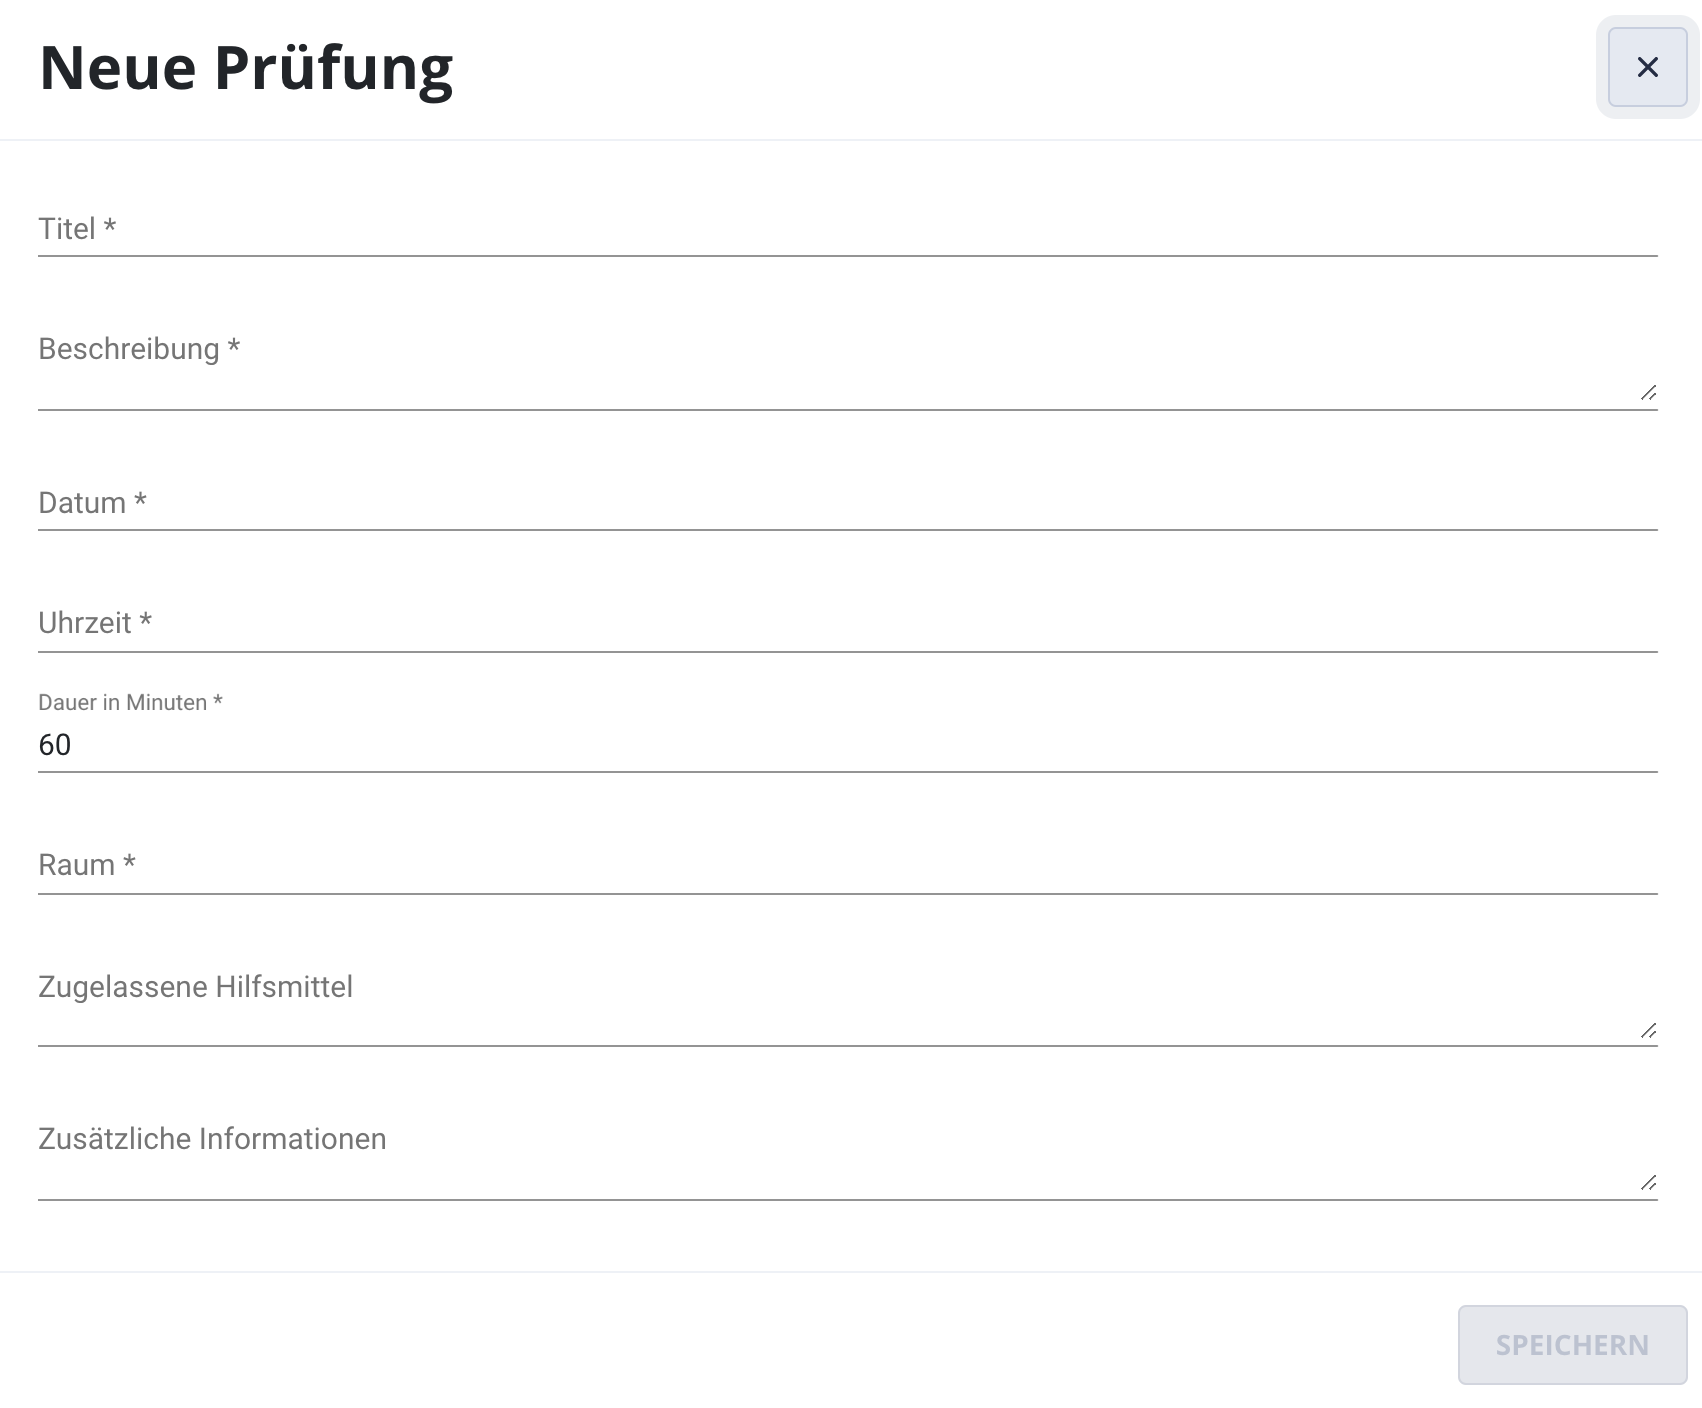
\includegraphics[width=.7\textwidth]{img/Pruefung_hinzugefuegen.png}
    \caption{Prüfungsmaske}
    \label{fig:pruefungsmaske}
\end{figure}
